% !TEX program = lualatex
\documentclass[a4paper,10pt,oneside,openany]{ltjsreport}
\usepackage[margin=21mm,top=19mm,bottom=20mm]{geometry}
\usepackage[haranoaji]{luatexja-preset}
\usepackage{amsmath,amssymb,graphicx,booktabs,longtable,xcolor,float}
\usepackage[unicode,colorlinks=true,linkcolor=blue!45!black,urlcolor=blue!45!black]{hyperref}
\usepackage{caption}
\captionsetup{font=small,labelfont=bf}
\setcounter{tocdepth}{0}
\setlength{\parskip}{0.45em}
\setlength{\parindent}{1em}
\raggedbottom
\newcommand{\sourcefile}[1]{{\small\texttt{\detokenize{#1}}}}
\begin{document}


\title{\Huge 実験6\\[0.6em]\LARGE 初期電子密度依存性\\[1em]\large 一次元HubbardモデルのUHF計算}

\author{保存結果の解析レポート}\date{2026年11月2日}\maketitle

\chapter*{概要}

ハミルトニアンと粒子数を固定し、一様型・反強磁性型・磁区壁型・ランダム型の初期密度を比較する。初期条件は物理パラメータではなく、自己無撞着解の探索経路を指定する。反強磁性型は今回の収束解の中で最も低エネルギーであり、一様型は1反復で収束するにもかかわらず高エネルギーにとどまる。収束と最小エネルギーは同義ではない。

対象は8ケース、保存図33枚である。収束は7ケース、未収束は1ケース。本書では生成物の種類ごとに章を設け、同じ条件のOBCとPBCを並べて読む。

\tableofcontents

\chapter{計算ログ：条件と最終結果}

\sourcefile{uhf_results.txt}

\section*{計算条件と量の定義}

$L=50$、$t=1$、温度 $T=0$、外部電場なし。全エネルギーと軌道エネルギーは $t$ を単位とする。
OBCは開放端、PBCはサイト50と1も接続する周期境界である。$N_e=N_\uparrow+N_\downarrow$、$\Delta N=N_\uparrow-N_\downarrow$ と定義する。
収束判定は混合前の密度残差 $r<10^{-10}$、最大反復回数は10000である。
表の「未」は未収束の最終再評価値であり、その桁数は精度保証ではない。

\begin{center}\small\setlength{\tabcolsep}{4pt}
\begin{longtable}{lrrrr}
\toprule
条件 & $N_e$ & $\Delta N$ & $U/t$ & mixing \\ \midrule
\endhead
uniform & 50 & 0 & 4 & 0.25 \\
AF & 50 & 0 & 4 & 0.25 \\
domain\_wall & 50 & 0 & 4 & 0.25 \\
random & 50 & 0 & 4 & 0.25 \\
\bottomrule\end{longtable}\end{center}

\section*{最終エネルギー}

$E=E_{\rm kin}+E_{\rm int}$、$E_{\rm int}=U\sum_i n_{i\uparrow}n_{i\downarrow}$。全エネルギーは占有軌道固有値の単純な総和ではなく、平均場の二重計数を除いた量である。

\begin{center}\small\setlength{\tabcolsep}{4pt}
\begin{longtable}{lrrrr}
\toprule
条件/境界 & 状態 & $E$ & $E_{\rm kin}$ & $E_{\rm int}$ \\ \midrule
\endhead
uniform/OBC & 収束 & -12.945484561 & -62.945484561 & 50.000000000 \\
uniform/PBC & 収束 & -13.703884440 & -63.703884440 & 50.000000000 \\
AF/OBC & 収束 & -23.013070704 & -43.110712440 & 20.097641737 \\
AF/PBC & 収束 & -23.455261995 & -43.889991764 & 20.434729770 \\
domain\_wall/OBC & 収束 & -22.634653771 & -42.591721328 & 19.957067557 \\
domain\_wall/PBC & 未 & -20.851780962 & -44.300241686 & 23.448460724 \\
random/OBC & 収束 & -22.634793115 & -42.593167746 & 19.958374631 \\
random/PBC & 収束 & -22.698428215 & -42.852011550 & 20.153583335 \\
\bottomrule\end{longtable}\end{center}

ハミルトニアンと粒子数を固定し、一様型・反強磁性型・磁区壁型・ランダム型の初期密度を比較する。初期条件は物理パラメータではなく、自己無撞着解の探索経路を指定する。反強磁性型は今回の収束解の中で最も低エネルギーであり、一様型は1反復で収束するにもかかわらず高エネルギーにとどまる。収束と最小エネルギーは同義ではない。

\section*{原資料と再利用}

出典は \sourcefile{results_vault/experiment_06/} 内の各条件/OBC・PBCのログ、CSV、PNG。\\ 補助資料は \sourcefile{experiment_conditions.md} と \sourcefile{uhf.jl}。値は保存済みの結果から採り、SCFを再実行していない。

条件名は原資料のディレクトリ名である。AFは実験2の再利用。

再利用データは独立した追加試行ではない。本書の解釈は保存された有限サイズ・UHF解の範囲に限る。

\chapter{密度CSV：電荷分布と二重占有}

\sourcefile{density_checkpoint.csv}

CSVの50サイトすべてから $q_i=n_{i\uparrow}+n_{i\downarrow}$、$m_i=n_{i\uparrow}-n_{i\downarrow}$、
$D=L^{-1}\sum_i n_{i\uparrow}n_{i\downarrow}$ を計算した。密度の各スピン成分は0以上1以下で、総和は指定した粒子数に一致することを確認した。未収束時のCSVは最後の混合密度を対角化して得た出力密度であり、固定点の密度とは限らない。

\begin{center}\small\setlength{\tabcolsep}{4pt}
\begin{longtable}{lrrrr}
\toprule
条件/境界 & 状態 & $\min q_i$ & $\max q_i$ & $D$ \\ \midrule
\endhead
uniform/OBC & 収束 & 1.000000 & 1.000000 & 0.250000 \\
uniform/PBC & 収束 & 1.000000 & 1.000000 & 0.250000 \\
AF/OBC & 収束 & 1.000000 & 1.000000 & 0.100488 \\
AF/PBC & 収束 & 1.000000 & 1.000000 & 0.102174 \\
domain\_wall/OBC & 収束 & 1.000000 & 1.000000 & 0.099785 \\
domain\_wall/PBC & 未 & 0.425770 & 1.574230 & 0.117242 \\
random/OBC & 収束 & 1.000000 & 1.000000 & 0.099792 \\
random/PBC & 収束 & 1.000000 & 1.000000 & 0.100768 \\
\bottomrule\end{longtable}\end{center}

一様型は各スピン0.5。反強磁性型は振幅0.1の交互変調。磁区壁型は $(-1)^i$ の後半（26--50サイト）の符号を反転し、平均を引いて粒子数を保つ。ランダム型はシード20261101で上下独立に一様乱数から平均を引き、最大絶対値で規格化して振幅0.1を与える。これらは実行ログに記録された具体的設定である。収束した結果の電荷密度はすべてほぼ1だが、スピン密度は大きく異なる。

\chapter{SCFエネルギー：反復による変化}

\sourcefile{scf_energy.png}

一様型に対する反強磁性型のエネルギー低下はOBCで約10.067586、PBCで約9.751378である。OBCの磁区壁型とランダム型はそれぞれ反強磁性型より約0.378417、0.378278高く、PBCのランダム型は約0.756834高い。異なる初期密度から異なる定常解に到達することが分かる。ただしヘッセ行列などの安定性解析はなく、各解を厳密な局所最小と断定はしない。

各図の横軸は反復回数、縦軸は各反復で評価した全エネルギーである。図ごとに軸範囲が異なるため、見かけの傾きだけを比較しない。最終ログ値は反復終了後の再評価であり、履歴の最終点とわずかに異なる場合がある。

\begin{center}\small\setlength{\tabcolsep}{4pt}
\begin{longtable}{lrrr}
\toprule
条件/境界 & 初回 $E$ & 最終 $E$ & 最後の履歴の $|\Delta E|$ \\ \midrule
\endhead
uniform/OBC & -12.945485 & -12.945485 & 履歴1点 \\
uniform/PBC & -13.703884 & -13.703884 & 履歴1点 \\
AF/OBC & -17.140038 & -23.013071 & $0$ \\
AF/PBC & -17.699645 & -23.455262 & $0$ \\
domain\_wall/OBC & -16.613794 & -22.634654 & $0$ \\
domain\_wall/PBC & -16.555858 & -20.851781 & $0$ \\
random/OBC & -12.284338 & -22.634793 & $0$ \\
random/PBC & -13.061296 & -22.698428 & $0$ \\
\bottomrule\end{longtable}\end{center}

\begin{figure}[H]\centering

\begin{minipage}{0.49\linewidth}\centering

\textbf{OBC：収束}\par

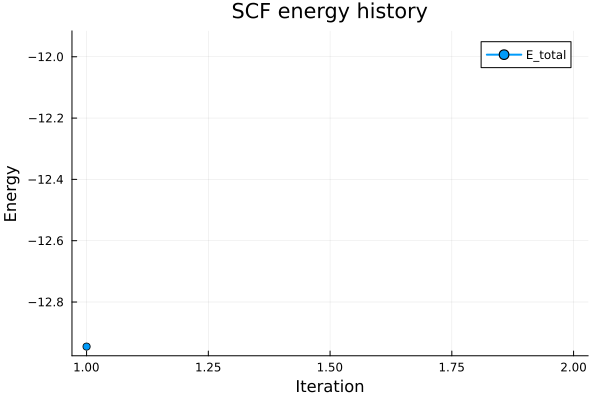
\includegraphics[width=\linewidth]{../../results_vault/experiment_06/uniform/OBC/scf_energy.png}

\end{minipage}\hfill%
\begin{minipage}{0.49\linewidth}\centering

\textbf{PBC：収束}\par

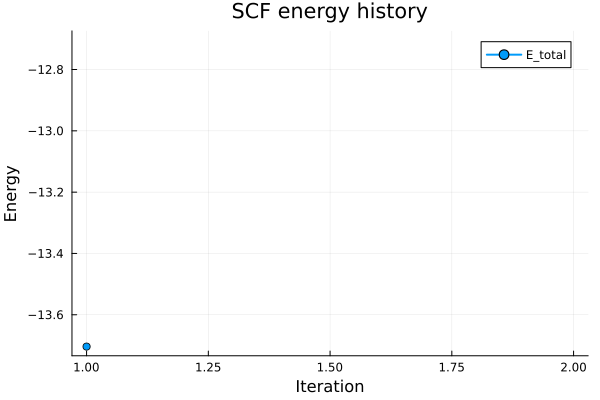
\includegraphics[width=\linewidth]{../../results_vault/experiment_06/uniform/PBC/scf_energy.png}

\end{minipage}

\caption{uniform。SCFエネルギーの比較。左：OBC、右：PBC。}\end{figure}

\begin{figure}[H]\centering

\begin{minipage}{0.49\linewidth}\centering

\textbf{OBC：収束}\par

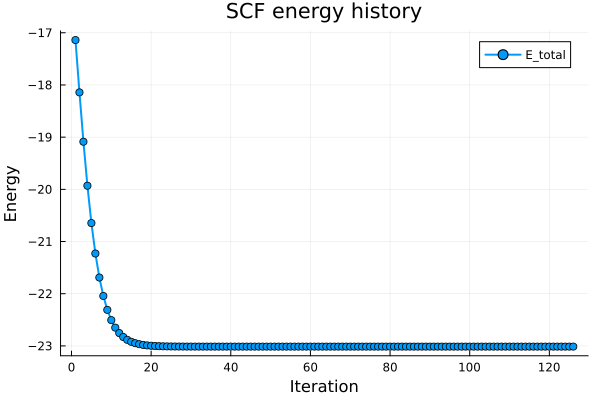
\includegraphics[width=\linewidth]{../../results_vault/experiment_06/AF/OBC/scf_energy.png}

\end{minipage}\hfill%
\begin{minipage}{0.49\linewidth}\centering

\textbf{PBC：収束}\par

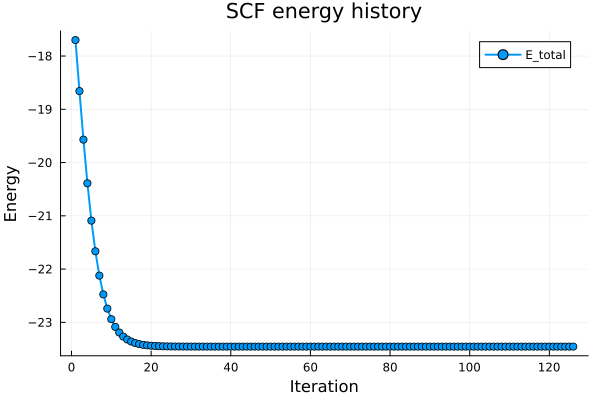
\includegraphics[width=\linewidth]{../../results_vault/experiment_06/AF/PBC/scf_energy.png}

\end{minipage}

\caption{AF。SCFエネルギーの比較。左：OBC、右：PBC。}\end{figure}

\begin{figure}[H]\centering

\begin{minipage}{0.49\linewidth}\centering

\textbf{OBC：収束}\par

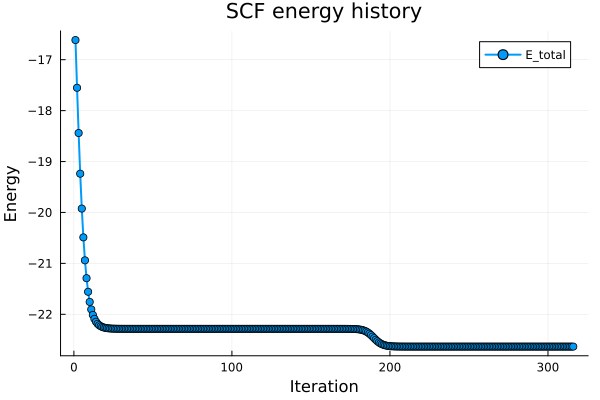
\includegraphics[width=\linewidth]{../../results_vault/experiment_06/domain_wall/OBC/scf_energy.png}

\end{minipage}\hfill%
\begin{minipage}{0.49\linewidth}\centering

\textbf{PBC：未収束・暫定}\par

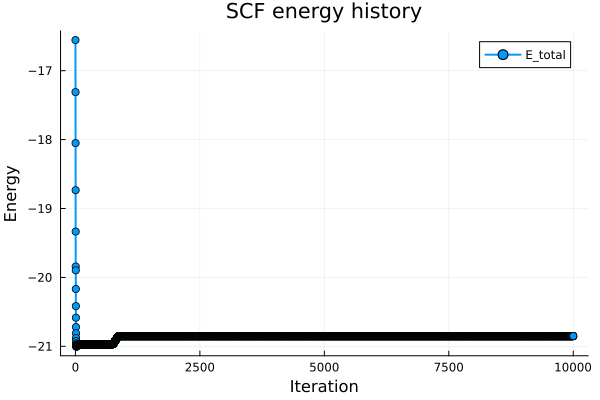
\includegraphics[width=\linewidth]{../../results_vault/experiment_06/domain_wall/PBC/scf_energy.png}

\end{minipage}

\caption{domain\_wall。SCFエネルギーの比較。左：OBC、右：PBC。}\end{figure}

\begin{figure}[H]\centering

\begin{minipage}{0.49\linewidth}\centering

\textbf{OBC：収束}\par

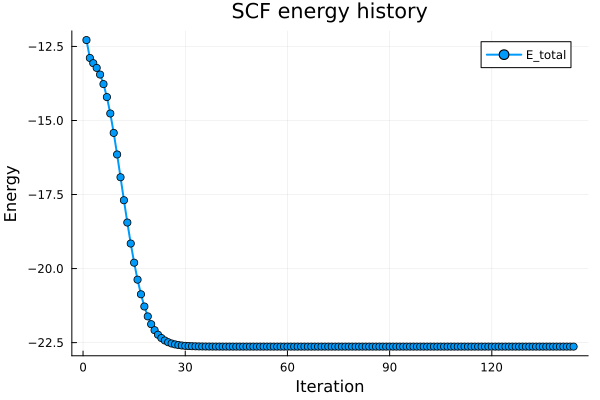
\includegraphics[width=\linewidth]{../../results_vault/experiment_06/random/OBC/scf_energy.png}

\end{minipage}\hfill%
\begin{minipage}{0.49\linewidth}\centering

\textbf{PBC：収束}\par

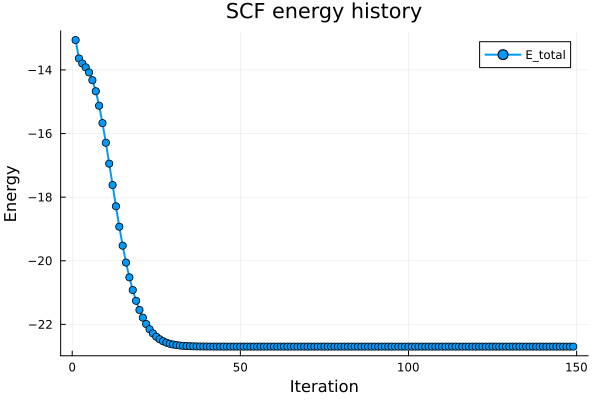
\includegraphics[width=\linewidth]{../../results_vault/experiment_06/random/PBC/scf_energy.png}

\end{minipage}

\caption{random。SCFエネルギーの比較。左：OBC、右：PBC。}\end{figure}

\chapter{SCF残差：自己無撞着性}

\sourcefile{scf_residual.png}

一様型は1反復、反強磁性型は126反復で収束する。ランダム型はOBCで144、PBCで149反復だが、磁区壁型のPBCは10000反復後も残差0.3281を残す。磁区壁型OBCは316反復で収束し、途中で残差が再増加する。初期状態に同じ名前を与えても、端の接続の有無により緩和経路は変わる。

残差は $r=\max_{i,\sigma}|F[n]_{i\sigma}-n_{i\sigma}|$。表は最終再評価値である。収束時には出力密度を採用してから再評価するため、履歴図の最後の残差とは同じとは限らない。

\begin{center}\small\setlength{\tabcolsep}{4pt}
\begin{longtable}{lrrr}
\toprule
条件/境界 & 状態 & 反復数 & 最終残差 \\ \midrule
\endhead
uniform/OBC & 収束 & 1 & $1.887\times10^{-14}$ \\
uniform/PBC & 収束 & 1 & $4.885\times10^{-15}$ \\
AF/OBC & 収束 & 126 & $3.266\times10^{-11}$ \\
AF/PBC & 収束 & 126 & $3.263\times10^{-11}$ \\
domain\_wall/OBC & 収束 & 316 & $3.326\times10^{-11}$ \\
domain\_wall/PBC & 未 & 10000 & $3.281\times10^{-1}$ \\
random/OBC & 収束 & 144 & $3.181\times10^{-11}$ \\
random/PBC & 収束 & 149 & $3.650\times10^{-11}$ \\
\bottomrule\end{longtable}\end{center}

\begin{figure}[H]\centering

\begin{minipage}{0.49\linewidth}\centering

\textbf{OBC：収束}\par

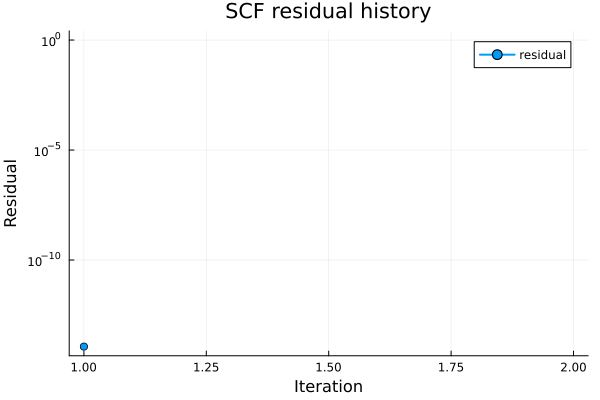
\includegraphics[width=\linewidth]{../../results_vault/experiment_06/uniform/OBC/scf_residual.png}

\end{minipage}\hfill%
\begin{minipage}{0.49\linewidth}\centering

\textbf{PBC：収束}\par

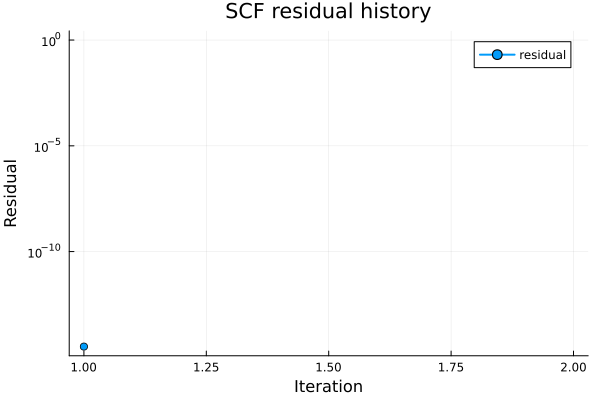
\includegraphics[width=\linewidth]{../../results_vault/experiment_06/uniform/PBC/scf_residual.png}

\end{minipage}

\caption{uniform。SCF残差の比較。左：OBC、右：PBC。}\end{figure}

\begin{figure}[H]\centering

\begin{minipage}{0.49\linewidth}\centering

\textbf{OBC：収束}\par

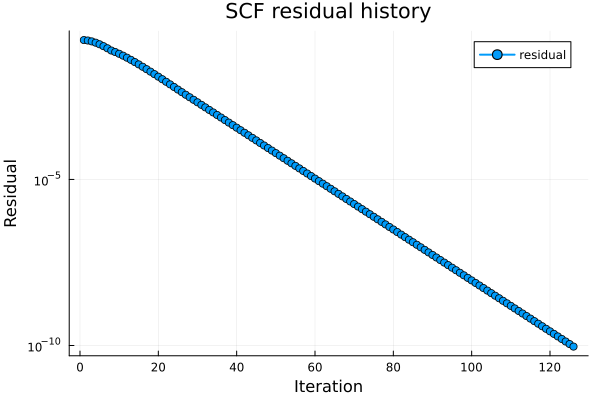
\includegraphics[width=\linewidth]{../../results_vault/experiment_06/AF/OBC/scf_residual.png}

\end{minipage}\hfill%
\begin{minipage}{0.49\linewidth}\centering

\textbf{PBC：収束}\par

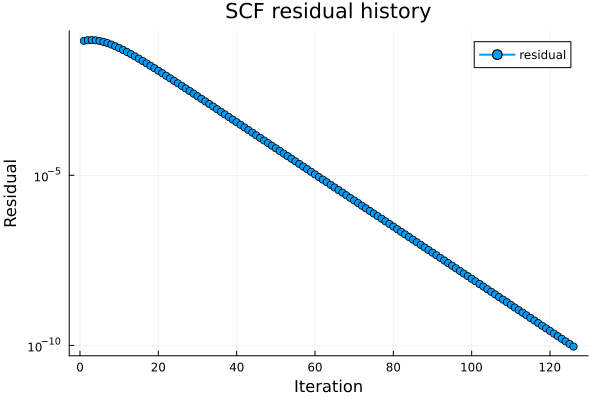
\includegraphics[width=\linewidth]{../../results_vault/experiment_06/AF/PBC/scf_residual.png}

\end{minipage}

\caption{AF。SCF残差の比較。左：OBC、右：PBC。}\end{figure}

\begin{figure}[H]\centering

\begin{minipage}{0.49\linewidth}\centering

\textbf{OBC：収束}\par

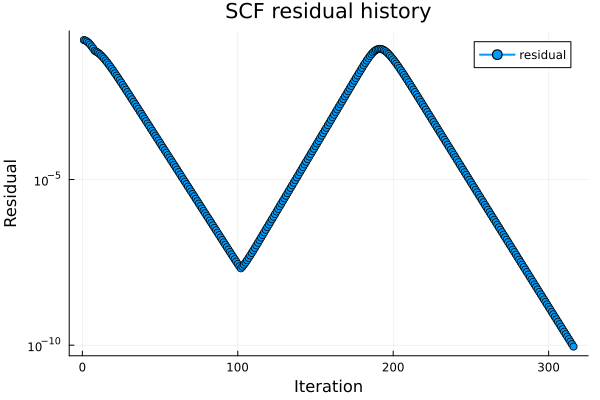
\includegraphics[width=\linewidth]{../../results_vault/experiment_06/domain_wall/OBC/scf_residual.png}

\end{minipage}\hfill%
\begin{minipage}{0.49\linewidth}\centering

\textbf{PBC：未収束・暫定}\par

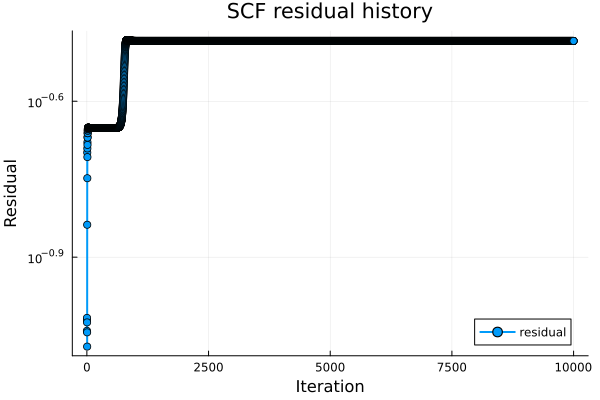
\includegraphics[width=\linewidth]{../../results_vault/experiment_06/domain_wall/PBC/scf_residual.png}

\end{minipage}

\caption{domain\_wall。SCF残差の比較。左：OBC、右：PBC。}\end{figure}

\begin{figure}[H]\centering

\begin{minipage}{0.49\linewidth}\centering

\textbf{OBC：収束}\par

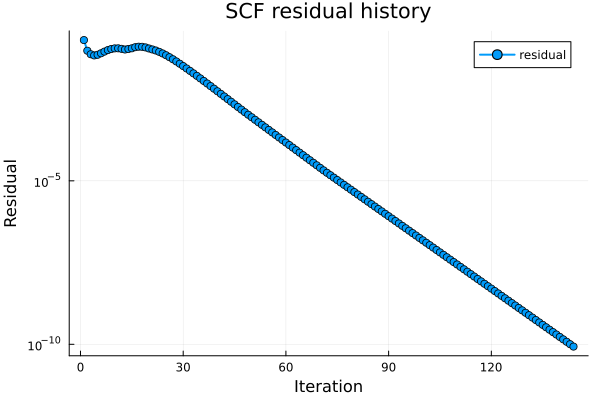
\includegraphics[width=\linewidth]{../../results_vault/experiment_06/random/OBC/scf_residual.png}

\end{minipage}\hfill%
\begin{minipage}{0.49\linewidth}\centering

\textbf{PBC：収束}\par

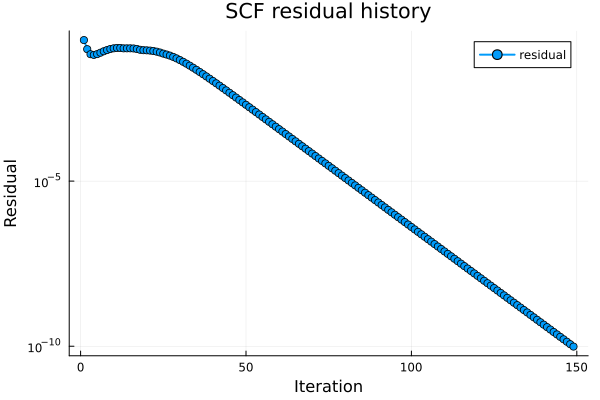
\includegraphics[width=\linewidth]{../../results_vault/experiment_06/random/PBC/scf_residual.png}

\end{minipage}

\caption{random。SCF残差の比較。左：OBC、右：PBC。}\end{figure}

\chapter{軌道エネルギー：準位構造}

\sourcefile{final_orbital_energies.png}

一様型の準位は非相互作用の準位を $U/2=2$ だけ上にずらした形で、反強磁性型に見られる大きな中央の分離はない。磁区壁型・ランダム型では端や中央付近の準位構造が反強磁性型と異なる。磁区壁型PBCの準位は未収束平均場のものであり、その形を安定な欠陥準位と確定してはならない。

横軸はエネルギー昇順の軌道番号、縦軸は $h_\sigma=h_0+U\operatorname{diag}(n_{\bar\sigma})$ の固有値である。固有値の数値ファイルは保存されていないため、図からの解釈は定性的なものに留める。未収束例をCSVから再対角化すると保存図とは異なる平均場になる可能性があり、本書ではその置換を行わない。

\begin{figure}[H]\centering

\begin{minipage}{0.49\linewidth}\centering

\textbf{OBC：収束}\par

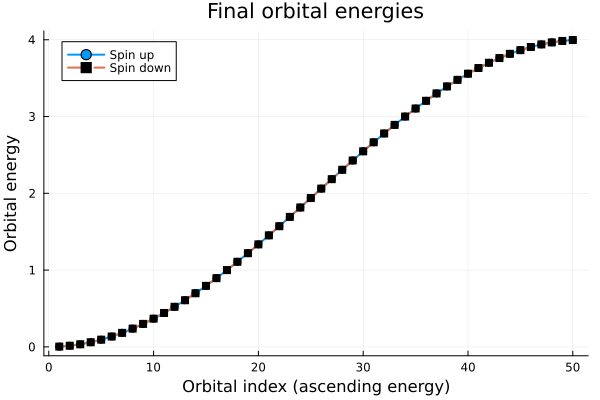
\includegraphics[width=\linewidth]{../../results_vault/experiment_06/uniform/OBC/final_orbital_energies.png}

\end{minipage}\hfill%
\begin{minipage}{0.49\linewidth}\centering

\textbf{PBC：収束}\par

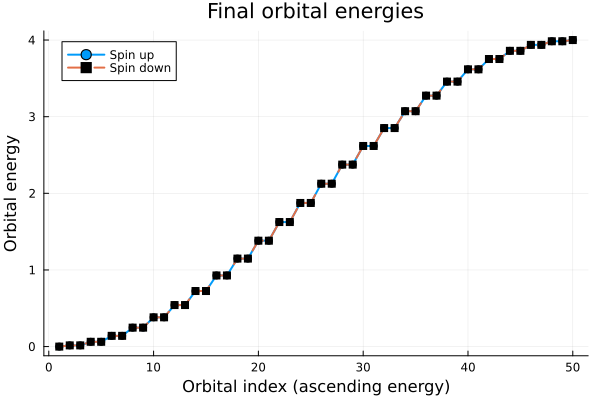
\includegraphics[width=\linewidth]{../../results_vault/experiment_06/uniform/PBC/final_orbital_energies.png}

\end{minipage}

\caption{uniform。軌道エネルギーの比較。左：OBC、右：PBC。}\end{figure}

\begin{figure}[H]\centering

\begin{minipage}{0.49\linewidth}\centering

\textbf{OBC：収束}\par

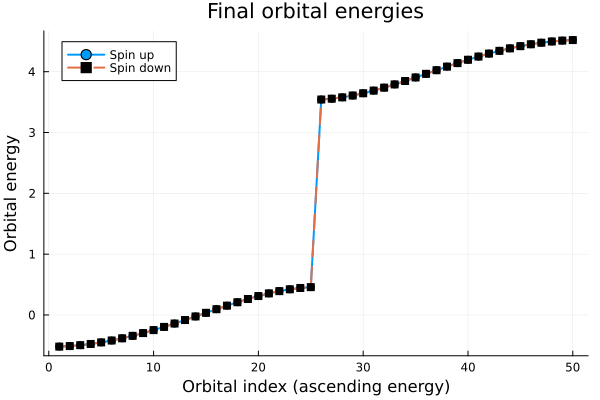
\includegraphics[width=\linewidth]{../../results_vault/experiment_06/AF/OBC/final_orbital_energies.png}

\end{minipage}\hfill%
\begin{minipage}{0.49\linewidth}\centering

\textbf{PBC：収束}\par

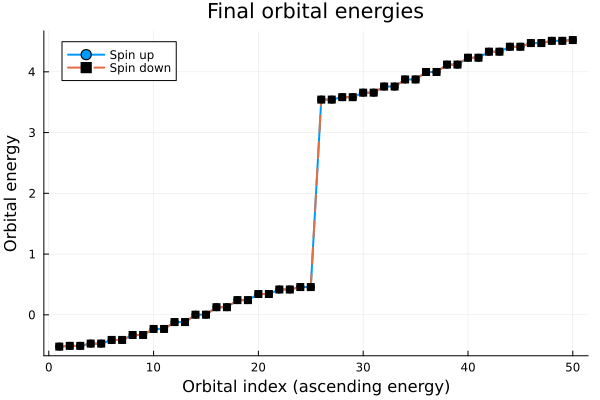
\includegraphics[width=\linewidth]{../../results_vault/experiment_06/AF/PBC/final_orbital_energies.png}

\end{minipage}

\caption{AF。軌道エネルギーの比較。左：OBC、右：PBC。}\end{figure}

\begin{figure}[H]\centering

\begin{minipage}{0.49\linewidth}\centering

\textbf{OBC：収束}\par

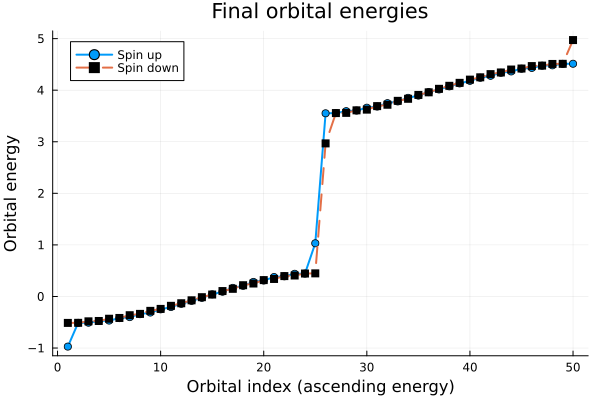
\includegraphics[width=\linewidth]{../../results_vault/experiment_06/domain_wall/OBC/final_orbital_energies.png}

\end{minipage}\hfill%
\begin{minipage}{0.49\linewidth}\centering

\textbf{PBC：未収束・暫定}\par

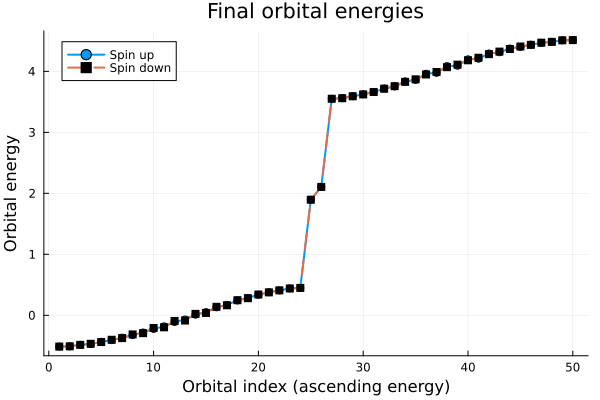
\includegraphics[width=\linewidth]{../../results_vault/experiment_06/domain_wall/PBC/final_orbital_energies.png}

\end{minipage}

\caption{domain\_wall。軌道エネルギーの比較。左：OBC、右：PBC。}\end{figure}

\begin{figure}[H]\centering

\begin{minipage}{0.49\linewidth}\centering

\textbf{OBC：収束}\par

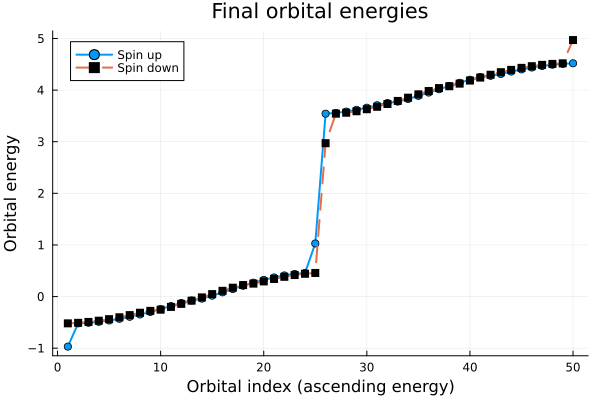
\includegraphics[width=\linewidth]{../../results_vault/experiment_06/random/OBC/final_orbital_energies.png}

\end{minipage}\hfill%
\begin{minipage}{0.49\linewidth}\centering

\textbf{PBC：収束}\par

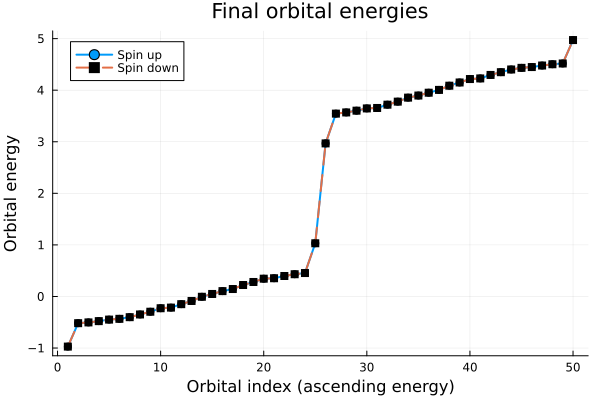
\includegraphics[width=\linewidth]{../../results_vault/experiment_06/random/PBC/final_orbital_energies.png}

\end{minipage}

\caption{random。軌道エネルギーの比較。左：OBC、右：PBC。}\end{figure}

\chapter{局所磁化：空間構造}

\sourcefile{final_magnetization.png}

一様型は磁化0、反強磁性型はほぼ一定振幅の交互磁化となる。磁区壁型OBCは $\overline{|m|}=0.774690$ と反強磁性型に近いが、$M_{\rm AF}=0.030759$ と小さい。逆位相の領域間で交互磁化が相殺するためである。ランダム型も局所振幅は保つが、符号配列の欠陥を残す。$M_{\rm AF}$ の小ささだけを局所モーメントの消失と解釈してはならない。

$\overline{|m|}=L^{-1}\sum_i|m_i|$、$M_{\rm AF}=|L^{-1}\sum_i(-1)^im_i|$ と定義する。$m_i$ はスピン密度差であり、$\langle S_i^z\rangle=m_i/2$ に対応する。全磁化は $\sum_i m_i=\Delta N$ と粒子数制約で固定される。

\begin{center}\small\setlength{\tabcolsep}{4pt}
\begin{longtable}{lrrr}
\toprule
条件/境界 & 状態 & $\overline{|m|}$ & $M_{\rm AF}$ \\ \midrule
\endhead
uniform/OBC & 収束 & 0.000000 & 0.000000 \\
uniform/PBC & 収束 & 0.000000 & 0.000000 \\
AF/OBC & 収束 & 0.773051 & 0.773051 \\
AF/PBC & 収束 & 0.768964 & 0.768964 \\
domain\_wall/OBC & 収束 & 0.774690 & 0.030759 \\
domain\_wall/PBC & 未 & 0.723322 & 0.030759 \\
random/OBC & 収束 & 0.774679 & 0.645940 \\
random/PBC & 収束 & 0.772243 & 0.461378 \\
\bottomrule\end{longtable}\end{center}

\begin{figure}[H]\centering

\begin{minipage}{0.49\linewidth}\centering

\textbf{OBC：収束}\par

\includegraphics[width=\linewidth]{../../results_vault/experiment_06/uniform/OBC/final_magnetization.png}

\end{minipage}\hfill%
\begin{minipage}{0.49\linewidth}\centering

\textbf{PBC：収束}\par

\includegraphics[width=\linewidth]{../../results_vault/experiment_06/uniform/PBC/final_magnetization.png}

\end{minipage}

\caption{uniform。局所磁化の比較。左：OBC、右：PBC。}\end{figure}

\begin{figure}[H]\centering

\begin{minipage}{0.49\linewidth}\centering

\textbf{OBC：収束}\par

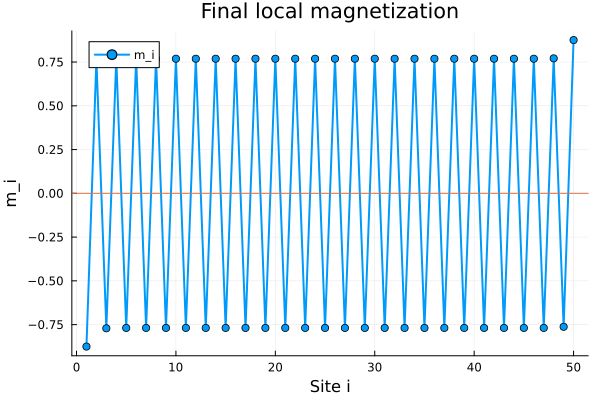
\includegraphics[width=\linewidth]{../../results_vault/experiment_06/AF/OBC/final_magnetization.png}

\end{minipage}\hfill%
\begin{minipage}{0.49\linewidth}\centering

\textbf{PBC：収束}\par

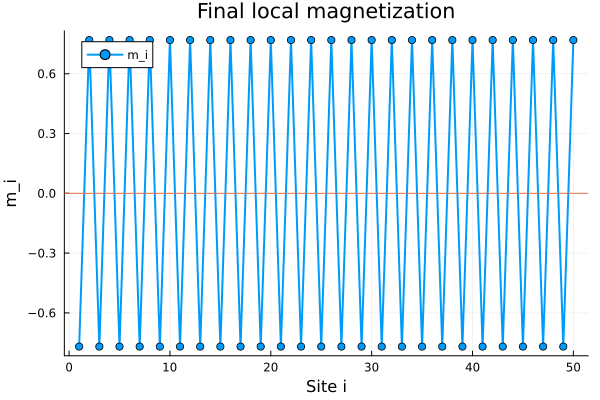
\includegraphics[width=\linewidth]{../../results_vault/experiment_06/AF/PBC/final_magnetization.png}

\end{minipage}

\caption{AF。局所磁化の比較。左：OBC、右：PBC。}\end{figure}

\begin{figure}[H]\centering

\begin{minipage}{0.49\linewidth}\centering

\textbf{OBC：収束}\par

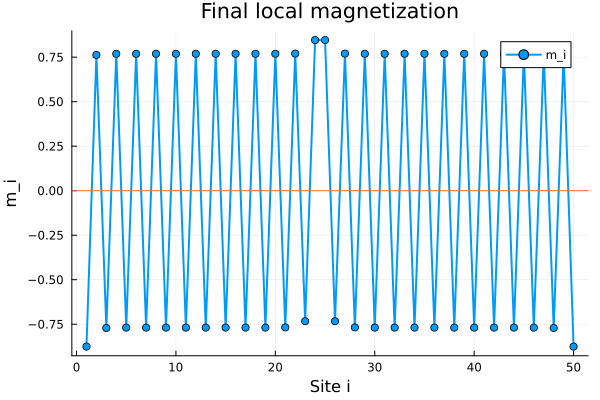
\includegraphics[width=\linewidth]{../../results_vault/experiment_06/domain_wall/OBC/final_magnetization.png}

\end{minipage}\hfill%
\begin{minipage}{0.49\linewidth}\centering

\textbf{PBC：未収束・暫定}\par

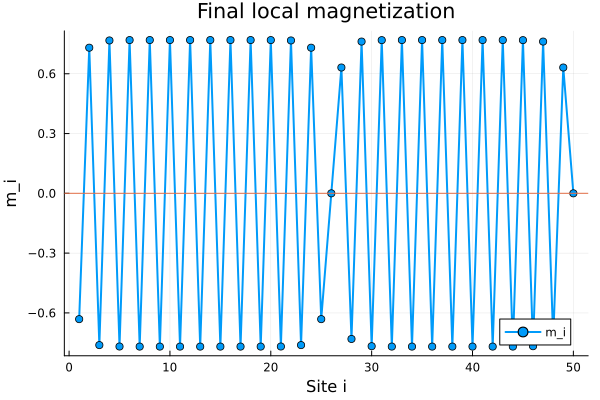
\includegraphics[width=\linewidth]{../../results_vault/experiment_06/domain_wall/PBC/final_magnetization.png}

\end{minipage}

\caption{domain\_wall。局所磁化の比較。左：OBC、右：PBC。}\end{figure}

\begin{figure}[H]\centering

\begin{minipage}{0.49\linewidth}\centering

\textbf{OBC：収束}\par

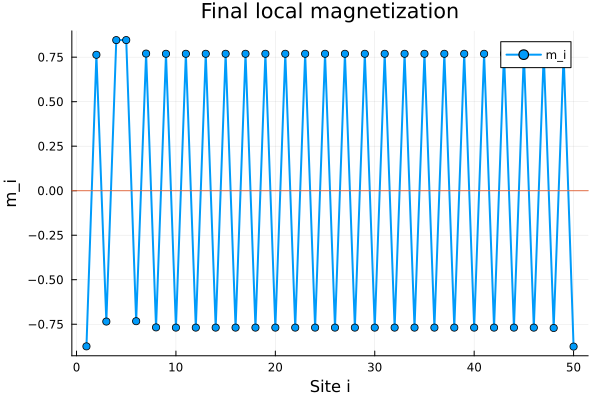
\includegraphics[width=\linewidth]{../../results_vault/experiment_06/random/OBC/final_magnetization.png}

\end{minipage}\hfill%
\begin{minipage}{0.49\linewidth}\centering

\textbf{PBC：収束}\par

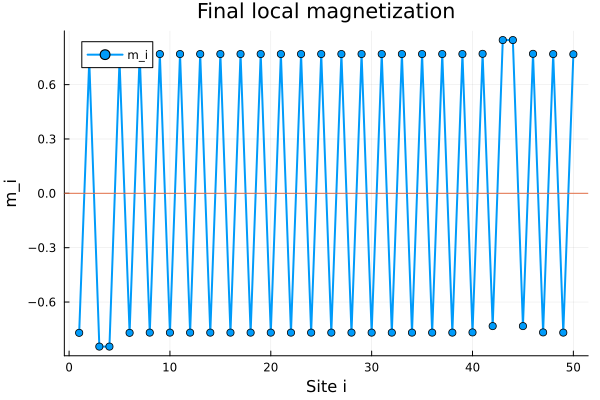
\includegraphics[width=\linewidth]{../../results_vault/experiment_06/random/PBC/final_magnetization.png}

\end{minipage}

\caption{random。局所磁化の比較。左：OBC、右：PBC。}\end{figure}

\chapter{境界条件による全エネルギー差}

\sourcefile{boundary_energy_difference.png}

$\Delta E_{\rm boundary}=E_{\rm PBC}-E_{\rm OBC}$ と定義する。負ならPBC、正ならOBCの保存された解の方が低エネルギーである。両方が収束した組だけを表と図で数値比較し、それ以外をNCとする。

差は一様型で $-0.758400$、反強磁性型で $-0.442191$、ランダム型で $-0.063635$ である。初期密度によって到達する解が変わるため、境界効果にも解の選択が混在する。ランダム型の差が小さいことを、系の境界依存性が普遍的に弱い証拠とはできない。磁区壁型の差はNCであり評価を保留する。

\begin{center}\small\setlength{\tabcolsep}{4pt}
\begin{longtable}{lrr}
\toprule
条件 & $\Delta E_{\rm boundary}$ & $\Delta E_{\rm boundary}/L$ \\ \midrule
\endhead
uniform & -0.758399879117 & -0.015167997582 \\
AF & -0.442191290827 & -0.008843825817 \\
domain\_wall & NC & NC \\
random & -0.063635099853 & -0.001272701997 \\
\bottomrule\end{longtable}\end{center}

\begin{figure}[H]\centering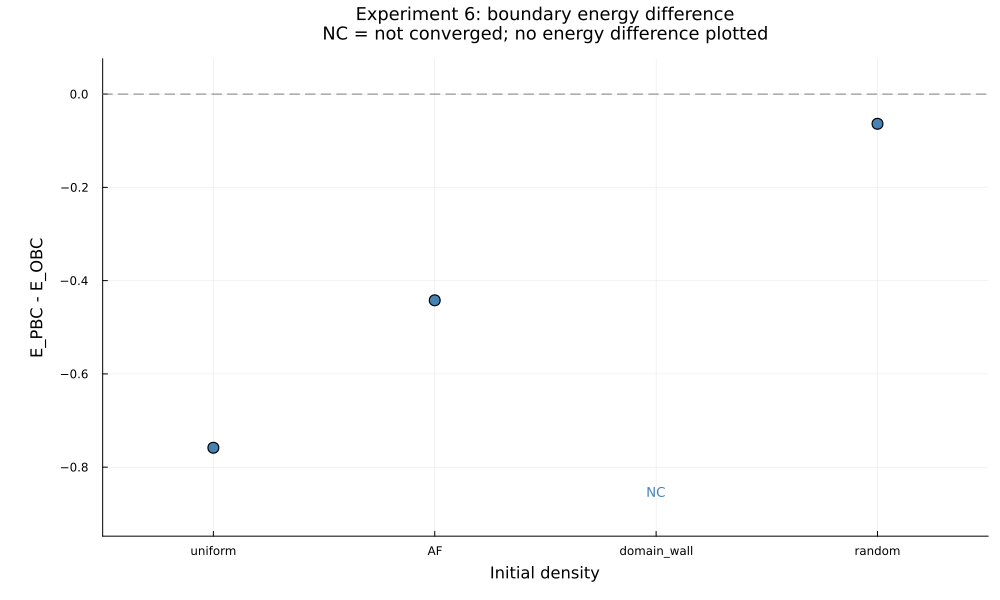
\includegraphics[width=0.9\linewidth]{../../results_vault/experiment_06/boundary_energy_difference.png}\caption{保存済みの境界エネルギー差。NCは未収束の組を示し、差が0であることを意味しない。}\end{figure}

\section*{結論と残された確認}

ハミルトニアンと粒子数を固定し、一様型・反強磁性型・磁区壁型・ランダム型の初期密度を比較する。初期条件は物理パラメータではなく、自己無撞着解の探索経路を指定する。反強磁性型は今回の収束解の中で最も低エネルギーであり、一様型は1反復で収束するにもかかわらず高エネルギーにとどまる。収束と最小エネルギーは同義ではない。

未収束ケースについては残差を満たす解を得た上で、複数の初期密度から同じ状態に到達するかを確認する必要がある。

サイズは50に固定しているため、境界効果と有限サイズ効果の切り分けには別サイズの結果が必要である。

\end{document}